\section{几乎必然收敛的判别}
\label{sec:rvconv-as-criteria}

怎样判断一列随机变量是否几乎必然收敛？定义要求几乎每条记录上的数列收敛，直接检查每条记录通常做不到。本节把问题翻译成事件的语言：误差最终小于$\varepsilon$，就是超差事件从某项起不再发生，也就是它只发生有限次。于是问题变成：一列事件在几乎每条记录上是否只发生有限次？

\subsection{无穷多次发生的事件}
\label{sec:rvconv-infinitely-often}

给定事件列$A_1,A_2,\dots$。一条记录$\omega$可能落在其中无穷多个事件里，也可能只落在有限个里。图~\ref{fig:rvconv-limsup-grid}画了四条记录：$\omega_1$落在所有偶数号事件里，$\omega_3$落在平方数号事件里，都是无穷多次；$\omega_2$只落在四个事件里；$\omega_4$从不落入。

\begin{BookInlineFigure}
 \centering
 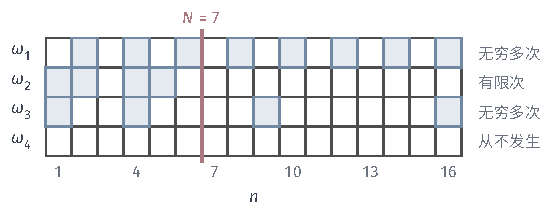
\includegraphics[width=94mm]{figures/07-probability/03-probability-limits/tikz/rvconv-limsup-grid/figure.pdf}
 \caption{事件的无穷次发生。每行是一条记录，第$n$列的浅蓝格表示该记录属于$A_n$。红线右侧是从$N=7$起的尾段：$\omega_1$与$\omega_3$在尾段中仍然出现，属于$\bigcup_{n\geq7}A_n$；$\omega_2$与$\omega_4$不属于。无论$N$取多大，$\omega_1$与$\omega_3$总留在尾段的并里。}
 \label{fig:rvconv-limsup-grid}
\end{BookInlineFigure}

“无穷多次”可以用可数次集合运算写出来。$\omega$落在无穷多个$A_n$中，等价于无论从哪一项$N$开始往后看，它都至少还落在一个$A_n$（$n\geq N$）中，即对每个$N$都有$\omega\in\bigcup_{n\geq N}A_n$。

\begin{definition}[事件的上极限与下极限]
\label{def:rvconv-limsup}
对事件列$(A_n)$，令
\begin{equation}
 \limsup_{n\to\infty}A_n=\bigcap_{N=1}^{\infty}\bigcup_{n\geq N}A_n,\qquad
 \liminf_{n\to\infty}A_n=\bigcup_{N=1}^{\infty}\bigcap_{n\geq N}A_n .
 \label{eq:rvconv-limsup}
\end{equation}
前者是$A_n$\term{无穷多次发生}（occurring infinitely often）的事件，也记作$\{A_n\ \text{i.o.}\}$；后者是从某项起$A_n$每次都发生的事件。
\end{definition}

两者都由可数次并与交得到，所以都是事件。取补集并交换并与交，得到
\[
 \Bigl(\limsup_{n\to\infty}A_n\Bigr)^{\mathrm{c}}=\bigcup_{N=1}^{\infty}\bigcap_{n\geq N}A_n^{\mathrm{c}}=\liminf_{n\to\infty}A_n^{\mathrm{c}} .
\]
右边说的是“存在$N$，从第$N$项起$A_n$不再发生”，也就是$A_n$只发生有限次。“无穷多次发生”与“最终不再发生”恰好互补。

尾段的并$\bigcup_{n\geq N}A_n$随$N$递减，由概率的连续性，
\begin{equation}
 \mathbb{P}\Bigl(\limsup_{n\to\infty}A_n\Bigr)=\lim_{N\to\infty}\mathbb{P}\Bigl(\bigcup_{n\geq N}A_n\Bigr) .
 \label{eq:rvconv-limsup-continuity}
\end{equation}
无穷多次发生的概率，就是“从第$N$项起至少再发生一次”的概率在$N\to\infty$时的极限。

\paragraph{应用于超差事件}
现在把$A_n$取为超差事件。对$\varepsilon>0$，记
\[
 A_n(\varepsilon)=\bigl\{\lvert X_n-X\rvert>\varepsilon\bigr\}.
\]
$\omega$上的数列$X_n(\omega)$收敛到$X(\omega)$，就是对每个$\varepsilon>0$，$\omega$只落在有限个$A_n(\varepsilon)$中。阈值有不可数多个，但$\varepsilon$越小超差事件越大，所以只需检查一列趋于零的阈值，例如$\varepsilon=1/k$。

\begin{theorem}[几乎必然收敛的事件判据]
\label{thm:rvconv-as-io}
以下三条等价：
\begin{enumerate}
 \item $X_n\xrightarrow{\mathrm{a.s.}}X$；
 \item 对每个$\varepsilon>0$，$\mathbb{P}\bigl(\limsup_nA_n(\varepsilon)\bigr)=0$；
 \item 对每个$\varepsilon>0$，
 \begin{equation}
  \lim_{N\to\infty}\mathbb{P}\Bigl(\sup_{n\geq N}\lvert X_n-X\rvert>\varepsilon\Bigr)=0 .
  \label{eq:rvconv-as-sup}
 \end{equation}
\end{enumerate}
并且在第2条中只需对$\varepsilon=1/k$（$k=1,2,\dots$）检查。
\end{theorem}

\begin{proof}
先写出不收敛的记录。$X_n(\omega)\not\to X(\omega)$当且仅当存在某个$k$，使$\lvert X_n(\omega)-X(\omega)\rvert>1/k$对无穷多个$n$成立。所以
\[
 \{X_n\not\to X\}=\bigcup_{k=1}^{\infty}\limsup_{n\to\infty}A_n(1/k) .
\]
右边是可数个事件的并，因此收敛集合是事件，这也补上了定义~\ref{def:rvconv-almost-sure}中可测性的说明。

1推2。对任意$\varepsilon>0$，取$k$使$1/k<\varepsilon$，则$A_n(\varepsilon)\subseteq A_n(1/k)$，于是$\limsup_nA_n(\varepsilon)$含于$\{X_n\not\to X\}$，概率为零。

2推1。只用$\varepsilon=1/k$：由上面的等式与可数次可加性，
\[
 \mathbb{P}(X_n\not\to X)\leq\sum_{k=1}^{\infty}\mathbb{P}\Bigl(\limsup_{n\to\infty}A_n(1/k)\Bigr)=0 .
\]

2与3等价。$\sup_{n\geq N}\lvert X_n-X\rvert>\varepsilon$当且仅当某个$n\geq N$使$\lvert X_n-X\rvert>\varepsilon$，所以
\[
 \Bigl\{\sup_{n\geq N}\lvert X_n-X\rvert>\varepsilon\Bigr\}=\bigcup_{n\geq N}A_n(\varepsilon) .
\]
由式~\eqref{eq:rvconv-limsup-continuity}，这个概率的极限就是$\mathbb{P}(\limsup_nA_n(\varepsilon))$。
\end{proof}

如果直接对所有$\varepsilon>0$取并，会得到不可数个事件的并，概率论不允许对它用可加性。单调性让我们只取可数个阈值，这是“阈值只需取一列趋于零的正有理数”的原因。

\paragraph{对照依概率收敛}
式~\eqref{eq:rvconv-as-sup}与依概率收敛的式~\eqref{eq:rvconv-in-probability}只差一个上确界：依概率收敛要求第$N$项的误差超标的概率趋于零，几乎必然收敛要求从第$N$项起的最大误差超标的概率趋于零。后者控制整个尾段，这再次说明它更强。

当误差的绝对值随$n$单调不增时，尾段的最大误差就是第$N$项的误差，两种收敛等价。累计最大值正是如此：$1-M_n$递减，超差事件随$n$缩小，尾段的并就是$A_N(\varepsilon)$。由式~\eqref{eq:rvconv-max-tail}，
\[
 \mathbb{P}\Bigl(\sup_{n\geq N}(1-M_n)>\varepsilon\Bigr)=(1-\varepsilon)^{N}\to0 ,
\]
这与第~\ref{sec:rvconv-almost-sure}小节的直接论证一致。移动区块则相反：每一层都铺满$[0,1)$，对$0<\varepsilon<1$和每个$N$，$\bigcup_{n\geq N}A_n(\varepsilon)=\Omega$，尾段并的概率恒为$1$。

\subsection{Borel–Cantelli引理}
\label{sec:rvconv-borel-cantelli}

上一小节把几乎必然收敛归结为$\mathbb{P}(\limsup_nA_n)=0$。尾段的并通常没有简单公式，但每个$A_n$的概率往往容易算。能否只用这些单项概率作出判断？答案取决于$\sum_n\mathbb{P}(A_n)$是否有限：有限时，用并集上界即可；无限时，还需要独立性。

\paragraph{概率可和的情形}
若各事件的概率之和有限，尾段的概率之和趋于零，尾段的并也就越来越不可能发生。

\begin{lemma}[Borel–Cantelli引理]
\label{lem:rvconv-borel-cantelli}
若事件列$(A_n)$满足$\sum_{n=1}^{\infty}\mathbb{P}(A_n)<\infty$，则
\begin{equation}
 \mathbb{P}\Bigl(\limsup_{n\to\infty}A_n\Bigr)=0 .
 \label{eq:rvconv-bc1}
\end{equation}
\end{lemma}

\begin{proof}
对每个$N$，$\limsup_nA_n\subseteq\bigcup_{n\geq N}A_n$。由可数次可加性给出的并集上界，
\[
 \mathbb{P}\Bigl(\limsup_{n\to\infty}A_n\Bigr)\leq\mathbb{P}\Bigl(\bigcup_{n\geq N}A_n\Bigr)\leq\sum_{n\geq N}\mathbb{P}(A_n) .
\]
右边是收敛级数的尾和，$N\to\infty$时趋于零，左边与$N$无关，所以为零。
\end{proof}

这个结论称为\term{Borel–Cantelli引理}（Borel–Cantelli lemma）。证明只用了并集上界，没有用到事件之间的任何关系，所以它不要求独立。级数收敛的直观含义是事件发生的平均次数有限：第~\ref{sec:rvconv-monotone}小节会证明发生次数$\sum_n\mathbf{1}_{A_n}$的期望等于$\sum_n\mathbb{P}(A_n)$，平均次数有限的计数几乎必然有限。

\paragraph{独立示性变量：概率可和}
回到独立示性变量$\xi_n=\mathbf{1}_{\{U_n<p_n\}}$，取$p_n=1/n^{2}$。级数
\[
 \sum_{n=1}^{\infty}\frac{1}{n^{2}}=\frac{\pi^{2}}{6}\approx1.645
\]
收敛，由引理~\ref{lem:rvconv-borel-cantelli}，几乎每条记录上只有有限个$\xi_n=1$。对这样的记录，从某项起$\xi_n=0$，所以$\xi_n\xrightarrow{\mathrm{a.s.}}0$。

这里的事件恰好独立，尾段并的概率也能精确算出。由独立性和补事件，对$N\geq2$，
\[
 \mathbb{P}\Bigl(\bigcup_{n=N}^{M}A_n\Bigr)=1-\prod_{n=N}^{M}\Bigl(1-\frac{1}{n^{2}}\Bigr)=1-\prod_{n=N}^{M}\frac{(n-1)(n+1)}{n\cdot n} .
\]

乘积是裂项的：分子中的$n-1$与前一项分母的$n$相消，$n+1$与后一项分母的$n$相消，只剩下首尾两个因子，
\[
 \prod_{n=N}^{M}\frac{(n-1)(n+1)}{n\cdot n}=\frac{N-1}{N}\cdot\frac{M+1}{M} .
\]
令$M\to\infty$，得到$\mathbb{P}\bigl(\bigcup_{n\geq N}A_n\bigr)=1/N$。$N=10$时它等于$0.1$，并集上界$\sum_{n\geq10}n^{-2}\approx0.105$，两者相当接近，见图~\ref{fig:rvconv-bc-unions}(a)。

\paragraph{概率不可和的情形}
级数发散时，并集上界失效。此时事件是否无穷多次发生取决于事件之间的关系。若各事件独立，发散的级数迫使它们无穷多次发生。

\begin{lemma}[独立事件的Borel–Cantelli引理]
\label{lem:rvconv-borel-cantelli-2}
若事件$A_1,A_2,\dots$相互独立，且$\sum_{n=1}^{\infty}\mathbb{P}(A_n)=\infty$，则
\begin{equation}
 \mathbb{P}\Bigl(\limsup_{n\to\infty}A_n\Bigr)=1 .
 \label{eq:rvconv-bc2}
\end{equation}
\end{lemma}

\begin{proof}
只需证明补事件的概率为零。由上一小节，补事件是
\[
 \Bigl(\limsup_{n\to\infty}A_n\Bigr)^{\mathrm{c}}=\bigcup_{N=1}^{\infty}\bigcap_{n\geq N}A_n^{\mathrm{c}} ,
\]
它是可数个事件的并，所以只需证明对每个$N$，
\[
 \mathbb{P}\Bigl(\bigcap_{n\geq N}A_n^{\mathrm{c}}\Bigr)=0 .
\]

相互独立事件的补事件仍相互独立。对$M\geq N$，记$p_n=\mathbb{P}(A_n)$，再用$1-x\leq\mathrm{e}^{-x}$（$x\in\mathbb{R}$），得到
\[
 \mathbb{P}\Bigl(\bigcap_{n=N}^{M}A_n^{\mathrm{c}}\Bigr)=\prod_{n=N}^{M}(1-p_n)\leq\exp\Bigl(-\sum_{n=N}^{M}p_n\Bigr) .
\]
级数发散，所以对固定的$N$，$\sum_{n=N}^{M}p_n\to\infty$（$M\to\infty$），右边趋于零。

$\bigcap_{n=N}^{M}A_n^{\mathrm{c}}$随$M$递减到$\bigcap_{n\geq N}A_n^{\mathrm{c}}$，由概率的连续性，后者的概率是左边的极限，等于零。
\end{proof}

不等式$1-x\leq\mathrm{e}^{-x}$把乘积化为和的指数：每个独立事件都有一份“不发生”的概率，它们相乘以后被发散的级数压到零。独立性用在第一个等号上，把交的概率写成乘积。

\paragraph{独立示性变量：概率不可和}
取$p_n=1/n$。$\sum_n1/n=\infty$，事件又相互独立，由引理~\ref{lem:rvconv-borel-cantelli-2}，几乎每条记录上都有无穷多个$\xi_n=1$，所以$\xi_n$几乎必然不收敛到$0$。另一方面，$\mathbb{P}(\xi_n=1)=1/n\to0$，$\mathbb{E}[\xi_n^{p}]=1/n\to0$，它依概率收敛、在每个$L^{p}$中收敛到$0$。这就补上了表~\ref{tab:rvconv-examples}中的第三行。

尾段并的概率同样可以精确计算。对$N\geq2$，乘积仍然裂项：
\[
 \mathbb{P}\Bigl(\bigcup_{n=N}^{M}A_n\Bigr)=1-\prod_{n=N}^{M}\frac{n-1}{n}=1-\frac{N-1}{M} .
\]
无论$N$多大，令$M\to\infty$它都趋于$1$。取$N=10$，$M=100$时已是$0.91$。图~\ref{fig:rvconv-bc-unions}(b)画出$N=10,100,1000$三条曲线：起点越晚，需要等得越久，但最终都要发生。

\begin{BookInlineFigure}
 \centering
 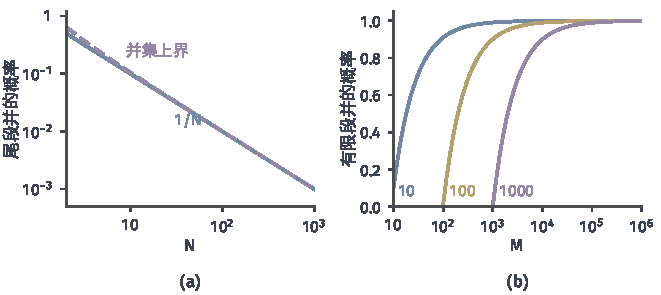
\includegraphics[width=112mm]{figures/07-probability/03-probability-limits/matplotlib/rvconv-bc-unions/figure.pdf}
 \caption{独立事件$A_n$尾段并的精确概率。(a)$\mathbb{P}(A_n)=1/n^{2}$：$\mathbb{P}(\bigcup_{n\geq N}A_n)=1/N$（蓝线）与并集上界$\sum_{n\geq N}n^{-2}$（紫色虚线），双对数坐标。(b)$\mathbb{P}(A_n)=1/n$：$\mathbb{P}(\bigcup_{n=N}^{M}A_n)=1-(N-1)/M$随$M$的变化，曲线旁的数字是起点$N$。}
 \label{fig:rvconv-bc-unions}
\end{BookInlineFigure}

图~\ref{fig:rvconv-bern-paths}从样本记录的角度看同一件事，画的是前$n$项中发生的次数$C_n=\sum_{k\leq n}\xi_k$。$p_n=1/n$时，计数在对数横轴上持续上升，期望是调和数$H_n\approx\ln n+0.577$，没有上限。$p_n=1/n^{2}$时，计数很早就停住，$10^{5}$项里只发生一两次。

\begin{BookInlineFigure}
 \centering
 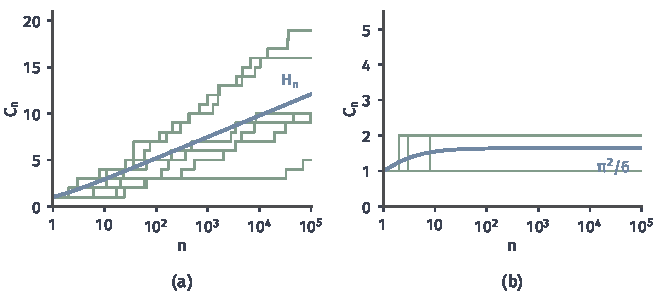
\includegraphics[width=112mm]{figures/07-probability/03-probability-limits/matplotlib/rvconv-bern-paths/figure.pdf}
 \caption{独立示性变量的累计发生次数$C_n=\sum_{k\leq n}\xi_k$，六条模拟记录（绿色，种子$2026$），横轴为对数刻度，$n\leq10^{5}$。蓝线是期望$\mathbb{E}[C_n]=\sum_{k\leq n}p_k$。(a)$p_n=1/n$，期望为调和数$H_n$，趋于无穷。(b)$p_n=1/n^{2}$，期望趋于$\pi^{2}/6\approx1.645$。}
 \label{fig:rvconv-bern-paths}
\end{BookInlineFigure}

两个引理合起来，对独立示性变量给出完整的回答：$\xi_n\xrightarrow{\mathrm{a.s.}}0$当且仅当$\sum_np_n<\infty$，而$\xi_n\xrightarrow{\mathbb{P}}0$当且仅当$p_n\to0$。$p_n\to0$但$\sum_np_n=\infty$的情形，例如$p_n=1/n$或$1/\sqrt{n}$，正好落在两者之间。它们还说明，独立事件的无穷多次发生只有两种可能：概率为$0$或为$1$。

\paragraph{去掉独立条件}
第二个引理的独立条件不能省略。取同一个事件重复：$A_n=A$对一切$n$成立，其中$0<\mathbb{P}(A)<1$。这时$\sum_n\mathbb{P}(A_n)=\infty$，但
\[
 \limsup_{n\to\infty}A_n=A,\qquad \mathbb{P}\Bigl(\limsup_{n\to\infty}A_n\Bigr)=\mathbb{P}(A)\in(0,1) .
\]
各项完全相关：在$A$上每次都发生，在$A$外从不发生。

依赖还可以把概率压到零。取$A_n=\{U<1/n\}$，$\sum_n1/n=\infty$，但这些事件递减，
\[
 \limsup_{n\to\infty}A_n=\bigcap_{n}\{U<1/n\}=\{U\leq0\},
\]
它的概率为零。所以概率发散时，没有独立性就什么也推不出：无穷多次发生的概率可以是$0$与$1$之间的任何值。第一个引理则对任何依赖结构都成立，这是两个方向在条件上的根本不对称。

\subsection{子列刻画}
\label{sec:rvconv-subsequence}

依概率收敛推不出几乎必然收敛，缺的是对整列的控制。但如果只看一部分项，跳过中间的项，超差概率就可能加起来有限。这是本小节的出发点：从依概率收敛的列中总能挑出几乎必然收敛的子列。

\begin{theorem}[几乎必然收敛的子列]
\label{thm:rvconv-subsequence}
若$X_n\xrightarrow{\mathbb{P}}X$，则存在子列$n_1<n_2<\cdots$，使$X_{n_k}\xrightarrow{\mathrm{a.s.}}X$。
\end{theorem}

\begin{proof}
由依概率收敛，对每个$k$，存在$N_k$使$n\geq N_k$时$\mathbb{P}(\lvert X_n-X\rvert>2^{-k})\leq2^{-k}$。递归地取$n_k\geq N_k$且$n_k>n_{k-1}$，令
\[
 E_k=\bigl\{\lvert X_{n_k}-X\rvert>2^{-k}\bigr\},\qquad \mathbb{P}(E_k)\leq2^{-k} .
\]

$\sum_k2^{-k}=1<\infty$，由引理~\ref{lem:rvconv-borel-cantelli}，$\mathbb{P}(\limsup_kE_k)=0$。对不在这个零概率事件中的$\omega$，存在$K(\omega)$，使$k\geq K(\omega)$时$\omega\notin E_k$，即
\[
 \lvert X_{n_k}(\omega)-X(\omega)\rvert\leq2^{-k},\qquad k\geq K(\omega) .
\]
右边趋于零，所以$X_{n_k}(\omega)\to X(\omega)$。
\end{proof}

阈值$2^{-k}$随$k$缩小，所以一个零概率例外集就同时照顾了所有精度，不需要再对$\varepsilon$取并。挑选子列的作用是让超差概率快速下降到可以求和，原列的超差概率可能下降得太慢。

\paragraph{移动区块的子列}
$B_n$依概率收敛到$0$，按定理应有几乎必然收敛的子列。每层取第一段即可：$n_k=k(k-1)/2+1$，
\[
 B_{n_k}=\mathbf{1}_{\{U<1/k\}} .
\]
对$U(\omega)>0$，$k>1/U(\omega)$以后$B_{n_k}(\omega)=0$，所以$B_{n_k}\xrightarrow{\mathrm{a.s.}}0$。图~\ref{fig:rvconv-subsequence}画出两条记录：原列在每层都碰到一次$1$，子列从某层起恒为零，而“某层”随记录改变。

\begin{BookInlineFigure}
 \centering
 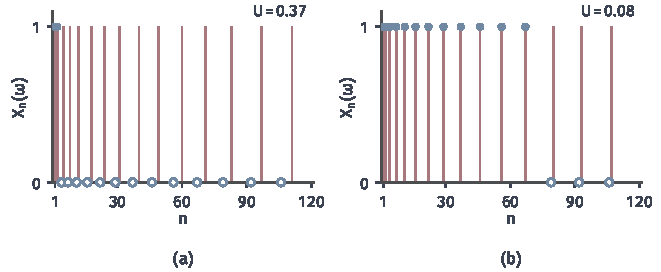
\includegraphics[width=112mm]{figures/07-probability/03-probability-limits/matplotlib/rvconv-subsequence/figure.pdf}
 \caption{移动区块的几乎必然收敛子列。红色竖线是原列$B_n(\omega)$取$1$的项，$n\leq120$；蓝点是子列$B_{n_k}=\mathbf{1}_{\{U<1/k\}}$（每层第一段）的取值，实心为$1$，空心为$0$。(a)$U=0.37$：子列只在$k=1,2$取$1$。(b)$U=0.08$：子列在$k\leq12$取$1$，此后恒为$0$。}
 \label{fig:rvconv-subsequence}
\end{BookInlineFigure}

这个子列的超差概率$1/k$加起来是发散的，它却几乎必然收敛：事件$\{U<1/k\}$递减，不独立。Borel–Cantelli引理是充分条件而不是必要条件。若按定理证明的办法挑选，会取到$k=2^{m}$那些层的第一段，超差概率$2^{-m}$可以求和。

\paragraph{独立示性变量的子列}
$p_n=1/n$时整列$\xi_n$不几乎必然收敛，但子列$n_k=k^{2}$的超差概率是$1/k^{2}$，可以求和。由引理~\ref{lem:rvconv-borel-cantelli}，$\xi_{k^{2}}\xrightarrow{\mathrm{a.s.}}0$。整列在几乎每条记录上无穷多次取$1$，但这些$1$几乎都落在跳过的项上。

\paragraph{完整的刻画}
一个几乎必然收敛的子列只是依概率收敛的一个推论，不足以反推整列依概率收敛。例如$X_{2m}=0$，$X_{2m-1}=\mathbf{1}_{\{U<1/2\}}$：偶数项的子列恒为零，而奇数项的超差概率恒为$1/2$，整列不依概率收敛到$0$。要刻画依概率收敛，必须对每一个子列都提出要求。

\begin{theorem}[依概率收敛的子列刻画]
\label{thm:rvconv-subsequence-criterion}
$X_n\xrightarrow{\mathbb{P}}X$当且仅当：对$(X_n)$的每个子列$(X_{n_k})$，都存在进一步的子列$(X_{n_{k_j}})$，使$X_{n_{k_j}}\xrightarrow{\mathrm{a.s.}}X$。
\end{theorem}

\begin{proof}
必要性。依概率收敛列的每个子列仍依概率收敛到$X$，对这个子列用定理~\ref{thm:rvconv-subsequence}即可。

充分性用反证法。若$X_n$不依概率收敛到$X$，则存在$\varepsilon>0$、$\delta>0$和子列$(n_k)$，使
\[
 \mathbb{P}\bigl(\lvert X_{n_k}-X\rvert>\varepsilon\bigr)\geq\delta,\qquad k=1,2,\dots
\]
按假设，它有进一步的子列几乎必然收敛到$X$，由定理~\ref{thm:rvconv-implications}也依概率收敛到$X$，其超差概率趋于零，与上式矛盾。
\end{proof}

前一个例子中，奇数项组成的子列没有任何进一步的子列收敛到$0$，所以条件不满足，这与整列不收敛一致。

\paragraph{几乎必然收敛没有这样的刻画}
移动区块满足定理~\ref{thm:rvconv-subsequence-criterion}中的条件：每个子列仍依概率收敛到$0$，因而有几乎必然收敛的进一步子列。但整列不几乎必然收敛。所以“每个子列都有收敛到$X$的进一步子列”这一条件，对几乎必然收敛不是充分的。

对由拓扑或距离定义的收敛，这一条件总是充分的：若$x_n\not\to x$，就有$x$的一个邻域和一个整个落在邻域外的子列，这个子列的任何进一步子列都不收敛到$x$。因此不存在一种距离，使随机变量按这种距离收敛恰好是几乎必然收敛。

依概率收敛则可以用一个平均量描述。对$0<\varepsilon\leq1$，把误差在$\varepsilon$处分开，并分别用$\min\{\lvert x\rvert,1\}\leq\varepsilon$（当$\lvert x\rvert\leq\varepsilon$）与$\min\{\lvert x\rvert,1\}\leq1$估计，再对超差事件用Markov不等式，得到
\[
 \varepsilon\,\mathbb{P}\bigl(\lvert X_n-X\rvert>\varepsilon\bigr)\leq\mathbb{E}\bigl[\min\{\lvert X_n-X\rvert,1\}\bigr]\leq\varepsilon+\mathbb{P}\bigl(\lvert X_n-X\rvert>\varepsilon\bigr) .
\]
所以$X_n\xrightarrow{\mathbb{P}}X$当且仅当$\mathbb{E}[\min\{\lvert X_n-X\rvert,1\}]\to0$。截去大于$1$的部分，是为了让稀有大值不影响这个平均，它衡量的只是“超差的机会”。

\paragraph{连续映射}
子列刻画的一个直接用途是传递依概率收敛。设$g:\mathbb{R}\to\mathbb{R}$连续，$X_n\xrightarrow{\mathbb{P}}X$，要证$g(X_n)\xrightarrow{\mathbb{P}}g(X)$。直接估计$\mathbb{P}(\lvert g(X_n)-g(X)\rvert>\varepsilon)$需要$g$的一致连续性，而$g$在整条实轴上未必一致连续。

用子列刻画则只需逐点的连续性。任取一个子列，它有进一步的子列几乎必然收敛到$X$；在这个子列上，对收敛的记录$\omega$，由$g$的连续性，$g(X_{n_{k_j}}(\omega))\to g(X(\omega))$，即$g(X_{n_{k_j}})\xrightarrow{\mathrm{a.s.}}g(X)$。由定理~\ref{thm:rvconv-subsequence-criterion}，$g(X_n)\xrightarrow{\mathbb{P}}g(X)$。例如$X_n\xrightarrow{\mathbb{P}}X$推出$X_n^{2}\xrightarrow{\mathbb{P}}X^{2}$。
